\chapter{Halbautomatische Erkennung zylindrischer Strukturen}
\label{cha:psoDomes}	
\dictum[deutsches Sprichwort]{Ein Bild sagt mehr als 1000 Worte.}	
	

\section{Motivation}

In diesem Kapitel soll das im Rahmen der Masterarbeit entwickelte Verfahren zur halbautomatischen Erfassung 
von zylindrischen Strukturen beschrieben werden. Ziel dieses Verfahrens ist es, die Aufw\"ande f\"ur das Ausmessen von Domstrukturen auf Spritzgu{\ss}teilen ma{\ss}geblich zu verringern (siehe Abschnitt \ref{problem}). 

Ein Dom ist, wie oben im Abschnitt \ref{dome} erl\"autert wurde, ein zylindrischer Vorsprung an einem Bauteil, der h\"aufig ein Befestigungselement aufnimmt. Da solche Dome die Fertigungskosten eines Spritzgu{\ss}teils erheblich steigern, ist es zur Absch\"atzung dieser Kosten notwendig, sowohl die Gesamtanzahl, als auch den Radius und die H\"ohe der einzelnen Zylinderstrukturen zu erfassen.

Das h\"andische Messverfahren, das im Abschnitt \ref{domeMeasure} beschrieben wurde, erlaubt das Messen der Domparameter durch das Platzieren eines parametrischen Zylinders auf einer Domstruktur und des Definierens der Zylinderh\"ohe und des Radius durch grafische Manipulatoren. 
Der parametrische K\"orper wird also durch die H\"ohe, den Radius und die sechs Freiheitsgrade seiner Starrk\"orpertransformation\footnote{Starrkörper besitzen sechs Freiheitsgrade: Sie können in drei Raumrichtungen
verschoben und um die drei Weltkoordinatensystemachsen rotiert werden.} eindeutig beschrieben. Eine zul\"assige Betrachtungsweise der Erfassung einer Domstruktur ist somit die Bestimmung von sinnvollen Werten für diese acht Parameter. Um das Messverfahren zu beschleunigen wurde ein Werkzeug entwickelt, das einerseits die Verschiebungs- und
Rotationswerte durch Analyse der Geometrie in der Umgebung einer Benutzereingabe und anderseits H\"ohe und Radius über heuristische Optimierung ermittelt.

Im Folgenden Abschnitt \ref{opti} wird kurz allgemein auf heuristische Optimierungsverfahren eingegangen. Danach wird in den Abschnitten  \ref{posTrafo} und \ref{goalFuction} beschrieben, wie die Parameter des Optimierungsproblems im einzelnen ermittelt werden. Abschnitt \ref{implPSO} geht auf die Implementierung und die Ergebnisse der Vorgehensweise ein.

\section{Heuristische Optimierung}
\label{opti}

Ein Optimierungsproblem im mathematischen Sinn ist die Aufgabe, für eine Funktion eine Menge aus Eingabewerten zu finden, so das der Funktion einen minimalen (oder maximalen) Wert annimmt, wobei in der Regel eine Beschr\"ankung der Eingabewerte vorliegt. Die beste Vorgehensweise hierf\"ur h\"angt von der Art der Bewertungsfunktion ab. Ist diese beispielsweise linear, lassen sich solche Probleme mit Hilfe von Verfahren, die auf dem  sogenannten Simplex-Algorithmus basieren, effizient l\"osen.

Handelt es sich nicht um lineare Zielfunktionen, sind analytische L\"osungsverfahren meistens sehr ineffizient und das systematische Durchsuchen des L\"oesungsraums ist aufgrund der Problemgr\"o{\ss}e nicht m\"oglich. F\"ur solche Probleme werden in der Informatik oft heuristische Optimierungsverfahren eingesetzt. Diese Verfahren generieren L\"osungen anhand einer definierten Vorgehensweise und verbessern diese suzessive, bis ein Abbruchkriterium, beispielsweise die Anzahl der Iterationen, erreicht ist. 

Im Gegensatz zu analytische Verfahren beinhaltet heuristische Optimierung immer die Nutzung von Zufallswerten, beispielweise beim Simulated Annealing, das im folgenden kurz erl\"autert wird, die initialen Punkte im L\"osungsraum. Dies hat zu Folge, das heuristische Optimierungsverfahren nichtdeterministisch sind, also das bei komplexen Problemen mit mehreren lokalen Optima unterschiedliche L\"osungen gefunden werden. 

Im Folgenden werden drei heuristische Optimierungsverfahren kurz erl\"autert: \textit{Simulated Annealing}, \textit{Evolution\"are Algorithmen} und \textit{Partikelschwarmoptimierung}. 

\textbf{\textit{Simulated Annealing}} (SA, siehe \cite{Kirkpatrik}) imitiert das Abkühlverhalten von Metallen. Kühlen diese langsam ab, haben die Atome ausreichend Zeit, sich zu ordnen und eine stabile Kristallstruktur zu bilden. Der Algorithmus betrachtet einen Punkt im n-dimensionalen L\"osungsraum, der schrittweise in Richtung eines Optimums bewegt wird. Vor jeder Bewegung wird die Zielposition bewertet: Fällt die Bewertung besser aus, als die aktuelle Position, wird die Bewegung durchgeführt. Fällt sie schlechter aus, wird sie nur mit einer gewissen Wahrscheinlichkeit durchgef\"uhrt, die mit jedem Schritt sukzessive verringert wird.Diese Wahrscheinlichkeit entspricht der Temperatur des metallurgischen Abkühlungsprozesses und dient dazu, lokale Minima zu \"uberwinden.

\begin{figure}[ht]
\centering
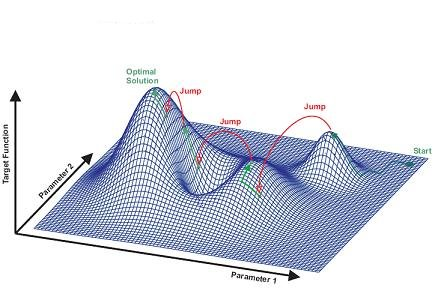
\includegraphics[width=10cm]{graphics/SimAnn.jpg}
\caption{Simulated Annealing in einem zweidimensionalen L\"osungsraum}
\label{fig6}
\end{figure}

\textbf{\textit{Evolution\"are Algorithmen} (EA)} sind eine Familie von Optimierungsverfahren, die sich das Prinzip der Selektion des Bestangepassten ("`\textit{Survival of the fittest}"') der nat\"urlichen Evolution zum Vorbild nehmen. Hierbei wird ein Punkt im L\"osungsraum als Individuum und eine Menge von Punkten als Population bezeichnet. Zu Beginn des Optimierungsverfahren wird der 
L\"osungsraum mit einer randomisierten Population "`bev\"olkert"', die zun\"achst mit einer Zielfunktion (in diesem Zusammenhang oft Fitness-Funktion) bewertet werden. Die am schlechtesten bewerteten Individuen werden verworfen, w\"arend aus den Verbliebenen die n\"achste Population durch Anwendung von sogenannten "`Evolutionären Operatoren"' erzeugt wird, beispielsweise Mutation
(leichtes Verändern eines Individuums) und Rekombination (Mischen der Gene zweier Individuen, oft auch als Crossover bezeichnet).
Dieser Zyklus aus Selektion, Crossover und Mutation wird solange wiederholt, bis ein vorgegebenes Abbruchkriterium (z. B. Anzahl der Generationen) erreicht ist.
Es werden die Hauptforschungsrichtungen Evolution\"are Programmierung (\cite{FogelAIsimEvo}), Genetische Algorithmen (\cite{GoldbergAISimEvo}) und Genetische Programmierung (\cite{KozaAIsimEvo}) unterschieden, die sich bez\"uglich der Datenstrukturen, Selektionsmethoden und der Operatoren unterscheiden.

Als \textbf{\textit{Partikelschwarmoptimierung} (PSO)} wird ein Optimierungsverfahren bezeichnet, das nach dem Vorbild nat\"urlichen Schwarmverhaltens von beispielsweise Fischen oder V\"ogeln eine L\"osung f\"ur das Optimierungsproblem sucht. Die hier beschriebene Version der PSO wurde zuerst 1995 in einer Forschungsarbeit von J. Kennedy and R. Eberhart präsentiert \cite{kennedyPSOConfPaper}. \"Ahnlich den evolution\"aren Algorithmen wird bei der Partikelschwarmoptimierung initial eine zuf\"allige  Menge vom Punkten im L\"osungsraum, die hier als Partikel bezeichnet werden, erzeugt. Der Partikelschwarm wird nun schrittweise durch den L\"osungsraum bewegt, wobei benachbarte Partikel vor jedem Schritt die beste Position, die ein Partikel bisher gefunden hat, austauschen k\"onnen. Welche Partikel miteinander kommunizieren k\"onnen wird durch die sogenannte Nachbarschaftstopologie bestimmt. 
Ein Partikel h\"alt somit zus\"atzlich zur Position $\vv{x}$ noch eine Bewegungsrichtung $\vv{v}$, die bisher beste gefundene Position als $\vv{p}_{best}$ und die beste Position seiner Umgebung als $\vv{n}_{best}$. Nach jedem Zeitschritt wird die Position und die Bewegungsrichtung (der Vektor $\vv{v}$ ist nicht normalisiert, er beinhaltet die Geschwindigkeit und Richtung) eines Partikels anhand folgender Formeln angepasst:

\begin{equation}
\vv{v}_{i,t+1} = \omega\cdot\vv{v}_{i,t}+c_{1}\cdot\vv{U}_{1}[0,1]\bigotimes(\vv{p}_{best,i,t})-\vv{x}_{i,t})
+c_{2}\cdot\vv{U}_{2}[0,1]\bigotimes(\vv{g}_{best,i,t})-\vv{x}_{i,t})
\end{equation}

\begin{equation}
\vv{x}_{i,t+1} = \vv{x}_{i,t} + \vv{v}_{i,t+1}
\end{equation}

Hierbei ist $t$ der Interationsz\"ahler, $\vv{U}_{k}[0,1]$ Zufallsvektoren und die Parameter $\omega$, $c_{1}$, $c_{1}$ bestimmen den Einflu{\ss}  der Position des vorigen Zeitschritts und der kognitiven und sozialen Komponenten.

Im Rahmen dieser Arbeit wird heuristische Optimierung benutzt, um f\"ur einen bereits ausgerichteten Zylinder H\"ohe, Radius und Rotation zu ermitteln. Dieses Problem ist nicht seperabel, d.h. einzelne Dimensionen des L\"osungsraums k\"onnen nicht oder nur begrenzt unabh\"angig voneinander untersucht werden. Dar\"uber hinaus gibt es im L\"osungsraum des Problems mehrere lokale Optima; es ist multimodal.

F\"ur die Implementierung des Optimierungsproblems wird Partikelschwarmoptimierung eingesetzt. Hierf\"ur wird ein Framework der Firma Teraport benutzt, das es erm\"oglicht, verschieden Optimierungsverfahren zu nutzen und Zielfunktionen zu implementieren.

\section{Ermittlung der Position und Ausrichtung einer Domstruktur}
\label{posTrafo}

Der relativ aufwendige Prozess des h\"andischen Ausmessens einer Domstruktur, der in Abschnitt \ref{domeMeasure} beschrieben wurde, kann zun\"achst beschleunigt werden, indem der Benutzer anstatt eine Punktwolke zu definieren, nur ein Dreieck der Oberfläche selektiert. Ausgehend von diesem Dreieck wird dann ein sogenannter Region Growing Prozess gestartet, der sukzessive benachbarte Dreiecke, die eine bestimmte Eigenschaft besitzen, einer Suchmenge hinzuf\"ugt.
Algorithmus \ref{alg:regionGrowing} beschreibt diese Vorgehensweise im allgemeinen.

\begin{algorithm}[H]
 \SetLine % For v3.9
 %\SetAlgoLined % For previous releases [?]
 \KwData{Dreieck $D_{S}$}
 \KwResult{$R$: Menge an Dreiecken mit einer bestimmten Eigenschaft}
 Erzeuge Stack $S$\;
 Füge $D_{S}$ zu $S$ hinzu\;
 \While{$S$ ist nicht leer}{
  Nehme oberstes Element $D$ vom Stack $S$\;
  Erzeuge Liste $N_{D}$ der Nachbarn von $D$\;
  \For{alle Dreiecke $D_{i}$ aus $N_{D}$}{
  \If{$D_{i}$ erf\"ullt die Zieleigenschaft und $D_{i}$ ist nicht in $R$ enthalten}{
     Lege $D_{i}$ auf $S$\;
   }
  }
  Erzeuge Liste $N_{D}$ der Nachbarn von $D$\;
  Füge $D$ zu $R$ hinzu\;
 }
 \caption{Region Growing}
 \label{alg:regionGrowing}
\end{algorithm}

Die gesuchte Eigenschaft ist hier eine \"ahnlich ausgerichtete Dreiecksnormale. Auf diese Weise kann, wenn der Benutzer ein Dreieck der planaren Zylinderoberseite selektiert, mit einem Klick die ganze Kappe ausgew\"ahlt werden.
Als Position des zu platzierenden Zylinders wird der Schwerpunkt der Zylinderkappe genutzt, der sich folgenderma{\ss}en berechnen l\"a{\ss}t:

\begin{equation}
v=\frac{\sum_{i}  a(v_{i})v_{i}}{\sum_{i}  a(v_{i})}
\end{equation}

Hier ist $v_{i}$ der Dreiecksmittelpunkt und  $a(v_{i})$ die Fläche des Dreiecks. Anschlie{\ss}end können die Scheitelpunkte der Dreiecke als Punktwolke interpretiert werden, f\"ur die mit Hilfe der Hauptkomponentenanalyse eine Best-Fitting Plane erzeugt werden, deren Normale die Rotation des Zylinders definiert. 

\subsection{Best-Fitting Plane mit Hauptkomponentenzerlegung}
\label{subsec:pca}

Eine \textit{Best-Fitting Plane} ist diejenige Ebene, die den aufsummierten orthogonalen Abstand einer Menge von Punkte zur Ebene minimiert (siehe Abbildung \ref{im:pca}). Eine Ebene kann geometrisch auf verschiedene Weise beschrieben werden. Im Rahmen dieser Arbeit wird die sogenannte Hessische Normalenform  zur Definition von Ebenen genutzt, die hierf\"ur einen Punkt ${P}$ und einen Normalenvektor $\vv{n}$ ben\"otigt.

\begin{figure}[ht]
\centering
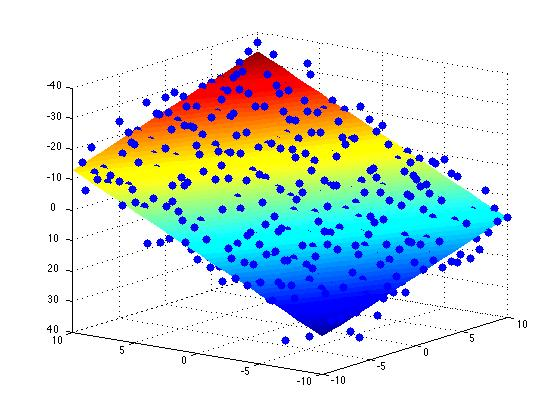
\includegraphics[width=10cm]{graphics/planefit.jpg}
\caption{Best Fitting Plane für eine dreidimensionale Punktwolke.}
\label{im:pca}
\end{figure}

Die \textit{Best-Fitting Plane} wird in dieser Arbeit mit der klassischen Methode, die auf der Hauptkomponentenanalyse (eng \textit{Principal Components Analysis}, kurz PCA) basiert, ermittelt. Dieses Verfahren basiert
auf der Kovarianzmatrix  ${Cov}_{p}$, die folgenderma{\ss}en aus der Punktemenge ${p_{i}}$ erzeugt wird:

\begin{equation}
{Cov_{p} =  \sum_{i} a(p_{i})(p_{i}-p)(p_{i}-p)^{T}}
\end{equation}

Der Punkt ${P}$ der Ebenengleichung ist der Schwerpunkt der Punktewolke $P$. Er wird durch das gewichtete Mittel der Ortsvektoren $\vv{p}_{i}$ der Punkte berechnet.

\begin{equation}
P=\frac{\sum_{i} \vv{p}_{i}}{i}}
\end{equation}

Die Ebenennormale $\vv{n}$ kann mittels Eigenvektorzerlegung von ${Cov}_{v}$ bestimmt werden: sie entspricht dem Eigenvektor, der mit dem kleinsten Eigenwert von ${Cov}_{v}$ korrespondiert. Wenn der kleinste Eigenwert 0 ist, bedeutet das, die Punktemenge ${P}$ koplanar ist. Da Eigenwertzerlegungen relativ aufwendig zu implementieren sind, wird hierf\"ur eine Bibliotheksfunktion verwendet. Der Vektor $\vv{n}$ kann einfach in eine Rotationsmatrix ${M}_{R}$ umgewandelt werden.

Das Verfahren kann einfach auf eine Menge von Dreiecken angewandt werden, indem die Vertices der Dreiecke als Punktewolke interpretiert werden. Der zu ermittelnde Zylinder kann dann im (gewichteten) Schwerpunkt (eng. \textit{Center of Cravity}, kurz COG) ${P_{T}}$ der Dreiecksmenge platziert werden.

\begin{equation}
P_{T}=\frac{\sum_{i} a(p_{i})\vv{p}_{i}}{\sum_{i} a(p_{i})}}
\end{equation}

Die Starrk\"orpertransformation (also die Positionierung und Ausrichtung im 3D-Raum) f\"ur den Zylinder ist durch von ${P_{T}}$ und ${M}_{R}$ vollst\"andig bestimmt. Die Ermittlung der H\"ohe und des Radius wird dann als mehrdimensionales Optimierungsproblem aufgefasst, f\"ur dessen L\"osung \textit{PSO} eingesetzt wird.

\section{Zielfunktion des Optimierungsproblems}
\label{goalFuction}

Kernidee der Zielfunktion ist die Nutzung einer virtuellen Messlehre. Eine  Lehre ist in der Technik ein Gerät, das für vorher festgelegte Maße und Formen ein Bezugsnormal darstellt, beispielsweise ein Messschieber oder ein Haarwinkel. Diese virtuelle Lehre ist ein degenerierter parametrischer Zylinder, der möglichst nah an die zu prüfende Bauteilgeometrie geschoben werden soll, ohne mit dieser zu kollidieren. Im folgenden wird der Messzylinder \textit{Pr\"ufzylinder}, die Bauteilgeometire \textit{model} genannt.

Der Pr\"uefzylinder besteht aus drei degenerierten Dreiecken, die zylindrisch angeordnet sind und in H\"ohe, Radius und Drehwinkel parametrisiert sind. Dies hat zum einen den Vorteil, das Kollisonsberechnungen mit drei degenerierten Dreiecken wenig aufwendig sind, und zum anderen, das mittels der Pr\"ufst\"abe auch mit St\"utzrippen ausgestattete Dome korrekt vermessen werden k\"onnen (siehe Abbildung \ref{im:messlehre}). Er wird initial korrekt ausgerichtet im Dreiecksschwerpunkt des Zylinderdeckels positioniert. 

\begin{figure}[ht]
\centering
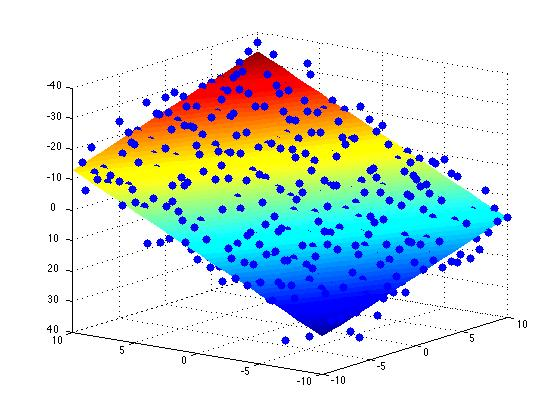
\includegraphics[width=10cm]{graphics/planefit.jpg}
\caption{Parametrischer Messzylinder f\"ur Bauteilgeometrie.}
\label{im:messlehre}
\end{figure}

\subsubsection{Kollisionsvermeidung}

Bei der Positionierung des Pr\"ufzylinders ist es vor allem wichtig, das die Pr\"ufgeometrie und das Modell nicht kollidieren. Hierf\"ur wird eine die properit\"are Implementierung der freien Kollisionsbibliothek Proximity Query Package (PQP) verwendet. Die Kolliosonspr\"ufung wird in Form eines Strafwertes in Bewertungsfunktion integriert: Kollidiert der Pr\"ufzylinder mit dem Model wird ein sehr hoher Strafwert zur\"uckgegeben.

\subsubsection{Ermittlung von H\"ohe und Radius}

Wenn die Pr\"ufgeometrie und das Model nicht kollidieren, werden die Werte f\"ur Radius, H\"ohe und Drehwinkel so interpretiert, das der Radius ${r}$ minimiert und die H\"ohe ${h}$ maximiert wird. Folgende Gleichung bestimmt den R\"uckgabewert ${V}$ bei nicht koolidierenden Geometrien:

\begin{equation}
{V=\lambda_{1}{r} + \lambda_{2}({-h})}
\end{equation}

Hierbei sind $\lambda_{1}$ und $\lambda_{2}$ Gewichtungsfaktoren, die  den Radius oder die H\"ohe st\"rker werten k\"onnen. Auf diese Weise kann das System so konfiguriert werden, das Dome mit Phasen an der Unterseite variabel erfasst werden k\"onnen: 

\begin{figure}[ht]
\centerline{
	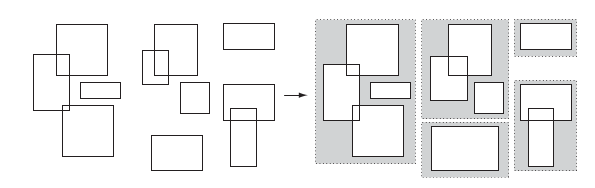
\includegraphics[width=0.7\columnwidth]{graphics/box.png}
}
\caption{Angephaster Zylinder mit unterschiedlichen $\lambda$-Werten.}
\label{im:messlehre}
\end{figure}

\vspace{1cm}

Algorithmus \ref{alg:goalFunction} fasst die Implementierung Zielfunktion  noch einmal zusammen:

\begin{algorithm}[H]
 \SetLine % For v3.9
 %\SetAlgoLined % For previous releases [?]
 \KwData{Bauteilgeometrie \textit{Model}, Höhe ${h}$, Radius ${r}$, Winkel ${a}$,$\lambda_{1}$, $\lambda_{2}$}
 \KwResult{Höhe und Radius}
 Erzeuge Pr\"ufgeometrie mit ${h}$, ${r}$, ${a}$\;
 Erzeuge PQP-Modell mit Pr\"ufgeometrie\;
 Pr\"ufe  Pr\"ufgeometrie und Modell auf Kollison\;
 \If{Pr\"ufgeometrie und Modell kollidieren}
 {
      return $10^9$\;
 }
 return ${V=\lambda_{1}{r} + \lambda_{2}({-h})}$
 \caption{Zielfunktion PSO}
 \label{alg:goalFunction}
\end{algorithm}


\section{Ergebnisse}
\label{resultsPSO}

Zur Evaluierung des implementierten Werkzeugs wurden einige Versuche mit verschieden Bauteilen durchgef\"uhrt.
Bei diesen Bauteilen handelt es sich zum einen um originale Fahrzeugdaten, zum anderen um eigens f\"ur die Domanylse konstruierte Modelle. Bei den folgenden Tests beziehen sich die Laufzeiten auf einen Intel Core2 Duo 6600 mit 2.4 GHz und 3 GB RAM. Als
Betriebssystem kam Windows XP (32 Bit), Service Pack 3 zum Einsatz.

Abbildung \ref{im:domes} zeigt verschiedene Domtypen, die mit dem implementierten Verfahren unterschiedlich gut erfasst werden k\"onnen:

\begin{figure}[ht]
    \centering 
    \subfigure[einfacher Dom]{
\includegraphics[width=0.19\textwidth]{graphics/dummy.jpg}} 
    \subfigure[Seitenrippen]{
\includegraphics[width=0.19\textwidth]{graphics/dummy.jpg}} 
    \subfigure[Schr\"age Unterseite]{
\includegraphics[width=0.19\textwidth]{graphics/dummy.jpg}} 
    \subfigure[Schr\"age Oberseite]{
\includegraphics[width=0.19\textwidth]{graphics/dummy.jpg}} 
       \subfigure[Runde Oberseite]{
\includegraphics[width=0.19\textwidth]{graphics/dummy.jpg}} 
\caption{Verschiedene Domtypen} 
\label{im:domes}
\end{figure} 

Ein einfacher Dom wie in der Abbildung \textit{a} ganz links kann problemlos erfasst werden; abh\"angig von den Werten f\"ur $\lambda_{1}$ und $\lambda_{2}$ wird die Bodenphase mit eingefasst oder nicht. Dome mit Seitenrippen wie in Abbildung \textit{b} kommen h\"aufig vor und k\"onnen gut erfasst werden (siehe Abbildung \ref{im:messlehre}). Bei Domen mit schr\"age Unterseiten funktioniert das Verfahren teilweise: Je nach Drehwinkel k\"onnen die Messst\"abe der Pr\"fgeometire bis zur unteren Kante reichen. Da die Erfassung der Domh\"ohen nur im Bereich von 10mm Schritten erfolgt, ist diese Ungenauigkeit in der Praxis akzeptabel. 

Dome mit schr\"ager Oberseite k\"onnen nur f\"ur sehr geringe Neigungswinkel korrekt erfasst werden, denn die Ausrichtung des Zylindersdeckels wird benutzt, um den Pr\"ufzylinder zu positionieren. Dies funktioniert nur, solange die Zylinderoberseite orthogonal zur Mittelachse der Domgeometrie steht (siehe Abbildung \ref{im:schraegDom}).

\begin{figure}[ht]
\centerline{
	
\includegraphics[width=0.19\columnwidth]{graphics/dummy.jpg}
}
\caption{Dome mit schr\"ager Oberseite.}
\label{im:schraegDom}
\end{figure}

Ein Dom mit runder Oberseite k\"onnen mit dem implementierten Verfahren nicht erfasst werden. Hier schl\"agt die Ermittlung der Position und der Rotation fehl, da das im Abschnitt \ref{posTrafo} vorgestellt wurde, keine planare Dreiecksmenge bestimmen kann. 

F\"ur die ersten drei in Abbildung \ref{im:domes} gezeigten Dome wurden mit dem umgesetzten Verfahren folgende Laufzeiten ben\"otigt:

\begin{center}
  \begin{tabular}{| l | c || r |}
    \hline
      & h\"andisches Ausmessen & halbautomatisches Verfahren \\ \hline
    Bauteil \textit{a} & 12s & 2300ms \\ \hline
    Bauteil \textit{b} & 8s  & 2500ms \\ \hline
    Bauteil \textit{c} & 8s & 2200ms \\
    \hline
  \end{tabular}
\end{center}

\section{Fazit und Ausblick}

Es wurde gezeigt das das vorgestellte halbautomatische Messverfahren eine wesentliche Verbesserung gegen\"uber der h\"andischen darstellt, da die Eigenschaften der am h\"aufigsten vorkommenden Domtypen in einem Bruchteil der Zeit erfasst werden k\"onnen. 
F\"ur Domstrukturen mit planarer Oberseite findet der Region-Growing Ansatz die Position und die Ausrichtung des Pr\"ufzylinders stabil und der gew\"ahlte Ansatz der heuristischen Optimierung l\"ost das restliche Optimierungsproblem zuverl\"assig. Die
Positionierungsergebnisse für den Pr\"ufzylinder wurden visuell überprüft und waren durchg\"angig plausibel. 
Es gab keine Durchdringungen und offensichtlich bessere Werte f\"ur H\"ohe und Radius war nicht auszumachen.

Das Verfahren funktioniert nur teilweise f\"r Domstrukturen mit sch\"rägem Boden. Dies k\"onnte insofern erweitert werden, dass die drei Messst\"abe des Pr\"ufzylinders mit jeweils einem H\"ohenparameter versehen werden. Diese Parameter k\"onnen als weitere Dimensionen f\"ur das Optimierungsproblem aufgefasst werden, wobei die Zielfunktion um diese drei Werte erweitert werden m\"usste.
Das Optimierungsverfahren w\"urde eine Stellunng des Pr\"ufzylinders liefern, in der ein Messstab die maximale H\"ohe liefert.

Bei Domen mit runden Oberseiten kann mit dem halbautomatischen Messwerkzeug kein Ergebnis gefunden werden. Dies kann gel\"ost werden, indem man die gesamte Starrk\"orpertransformation als achtdimensionales Optimierungsproblem auffasst. Dabei ist das Problem zu lösen, dass die Dimensionalität des Suchraums weiter ansteigt und damit der Aufwand f\"ur die Berechnung drastisch erh\"oht wird.





